\subsection{Упражнение 1}

Запустите и прослушайте примеры в файле chap03.ipynb. В примере с утечкой попробуйте заменить окно Хэмминга одним из других окон, предоставляемых NumPy, и посмотрите, как они влияют на утечку.

Если длительность кратна периоду, то начало и конец отрезка совпадают, и мы получаем минимальную утечку.

\begin{lstlisting}[language=Python]
from thinkdsp import SinSignal

signal = SinSignal(freq=440)
duration = signal.period * 30
wave = signal.make_wave(duration)
wave.plot()
decorate(xlabel='Time (s)')

spectrum.plot(high=880)
\end{lstlisting}

\begin{figure}[H]
	\begin{center}
		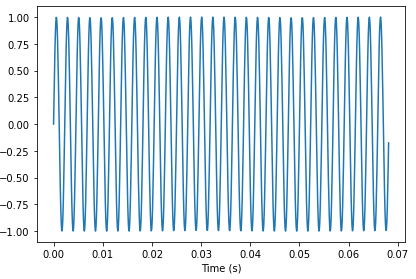
\includegraphics[scale=1]{fig/lab03/lab03_01.png}
		\caption{Рассматриваемый сигнал}
	\end{center}
\end{figure}

\begin{lstlisting}[language=Python]
spectrum = wave.make_spectrum()
spectrum.plot(high=880)
decorate(xlabel='Frequency (Hz)', ylabel='Amplitude')
\end{lstlisting}

\begin{figure}[H]
	\begin{center}
		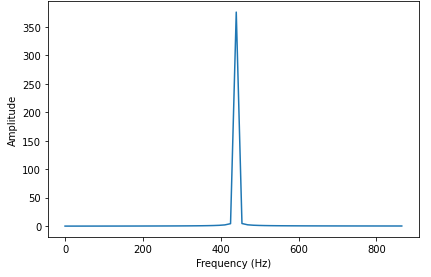
\includegraphics[scale=1]{fig/lab03/lab03_02.png}
		\caption{Спектр рассматриваемого сигнала}
	\end{center}
\end{figure}

Если продолжительность не кратна периоду, утечка довольно плохая.

\begin{lstlisting}[language=Python]
duration = signal.period * 30.25
wave = signal.make_wave(duration)
wave.plot()
decorate(xlabel='Time (s)')
\end{lstlisting}

\begin{figure}[H]
	\begin{center}
		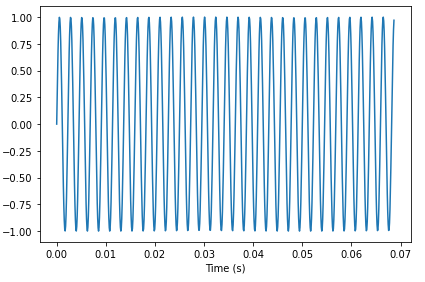
\includegraphics[scale=1]{fig/lab03/lab03_03.png}
		\caption{Рассматриваемый сигнал}
	\end{center}
\end{figure}

\begin{lstlisting}[language=Python]
spectrum = wave.make_spectrum()
spectrum.plot(high=880)
decorate(xlabel='Frequency (Hz)')
\end{lstlisting}

\begin{figure}[H]
	\begin{center}
		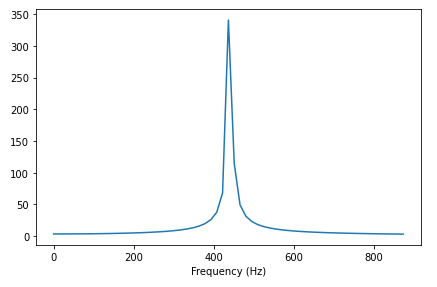
\includegraphics[scale=1]{fig/lab03/lab03_04.png}
		\caption{Спектр рассматриваемого сигнала}
	\end{center}
\end{figure}

Работа с окнами помогает (но обратите внимание, что она снижает общую энергию).

\begin{lstlisting}[language=Python]
wave.hamming()
spectrum = wave.make_spectrum()
spectrum.plot(high=880)
decorate(xlabel='Frequency (Hz)')
\end{lstlisting}

\begin{figure}[H]
	\begin{center}
		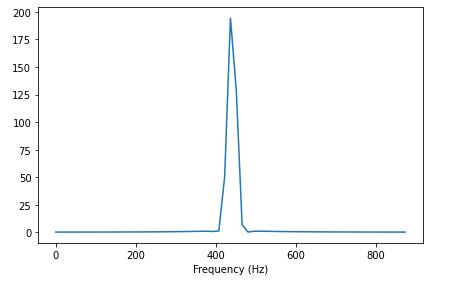
\includegraphics[scale=1]{fig/lab03/lab03_05.png}
		\caption{Спектр сигнала с применение окна Хээминга}
	\end{center}
\end{figure}

Если вы вслепую вычислите ДПФ непериодического сегмента, вы получите «размытие движения».

\begin{lstlisting}[language=Python]
signal = Chirp(start=220, end=440)
wave = signal.make_wave(duration=1)
spectrum = wave.make_spectrum()
spectrum.plot(high=700)
decorate(xlabel='Frequency (Hz)')
\end{lstlisting}

\begin{figure}[H]
	\begin{center}
		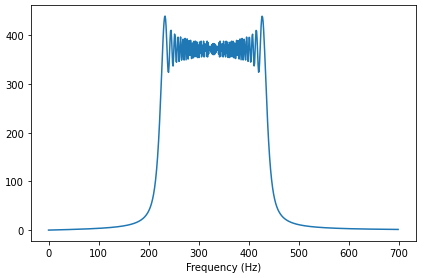
\includegraphics[scale=1]{fig/lab03/lab03_06.png}
		\caption{Спектр сигнала}
	\end{center}
\end{figure}

Спектрограмма — это визуализация кратковременного ДПФ, позволяющая увидеть, как спектр меняется во времени.

\begin{lstlisting}[language=Python]
def plot_spectrogram(wave, seg_length):
    """
    """
    spectrogram = wave.make_spectrogram(seg_length)
    print('Time resolution (s)', spectrogram.time_res)
    print('Frequency resolution (Hz)', spectrogram.freq_res)
    spectrogram.plot(high=700)
    decorate(xlabel='Time(s)', ylabel='Frequency (Hz)')
    
signal = Chirp(start=220, end=440)
wave = signal.make_wave(duration=1, framerate=11025)
plot_spectrogram(wave, 512)

Time resolution (s) 0.046439909297052155
Frequency resolution (Hz) 21.533203125
\end{lstlisting}

\begin{figure}[H]
	\begin{center}
		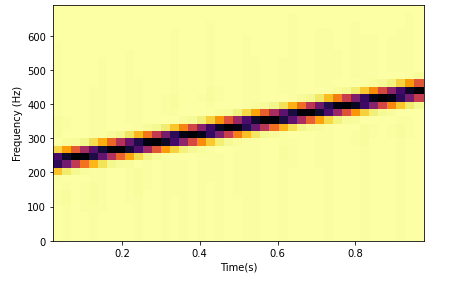
\includegraphics[scale=1]{fig/lab03/lab03_07.png}
		\caption{КПФ сигнала}
	\end{center}
\end{figure}

Если вы увеличите длину сегмента, вы получите лучшее разрешение по частоте, худшее разрешение по времени.

\begin{lstlisting}[language=Python]
plot_spectrogram(wave, 1024)

Time resolution (s) 0.09287981859410431
Frequency resolution (Hz) 10.7666015625
\end{lstlisting}

\begin{figure}[H]
	\begin{center}
		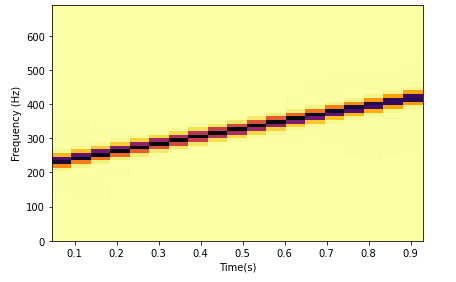
\includegraphics[scale=1]{fig/lab03/lab03_08.png}
		\caption{КПФ измененного сигнала}
	\end{center}
\end{figure}

Если вы уменьшите длину сегмента, вы получите лучшее временное разрешение, худшее разрешение по частоте.

\begin{lstlisting}[language=Python]
plot_spectrogram(wave, 256)

Time resolution (s) 0.023219954648526078
Frequency resolution (Hz) 43.06640625
\end{lstlisting}

\begin{figure}[H]
	\begin{center}
		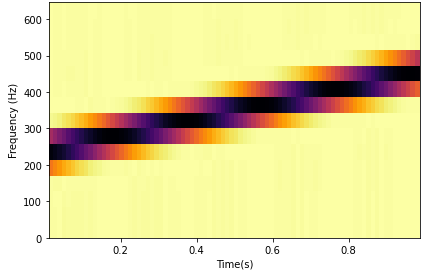
\includegraphics[scale=1]{fig/lab03/lab03_09.png}
		\caption{КПФ измененного сигнала}
	\end{center}
\end{figure}


\subsection{Упражнение 2}


Создадим класс SawtoothChirp, расширяющий Chirp и переопределяющий evaluate для генерации пилообразного сигнала с линейно увеличивающейся (или уменьшающейся) частотой

\begin{lstlisting}[language=Python]
from thinkdsp import Chirp
from thinkdsp import normalize, unbias

PI2 = 2 * np.pi

class SawtoothChirp(Chirp):

    def evaluate(self, ts):
        freqs = np.linspace(self.start, self.end, len(ts))
        dts = np.diff(ts, prepend=0)
        dphis = PI2 * freqs * dts
        phases = np.cumsum(dphis)
        cycles = phases / PI2
        frac, _ = np.modf(cycles)
        ys =  normalize(unbias(frac), self.amp)
        return ys
\end{lstlisting}

Протестируем полученный класс. Создадим пилообразный сигнал от 1318Hz до частоты 5274Hz

\begin{lstlisting}[language=Python]
sig = SawtoothChirp(1318, 5274)
w = sig.make_wave(duration = 4, framerate = 10000)
w.apodize()
w.make_audio()
\end{lstlisting}

Можно услышать биения

Теперь построим и распечатаем спектограмму этого сигнала

\begin{lstlisting}[language=Python]
sp = w.make_spectrogram(seg_length = 512)
sp.plot(high = 7000)
\end{lstlisting}

\begin{figure}[H]
	\begin{center}
		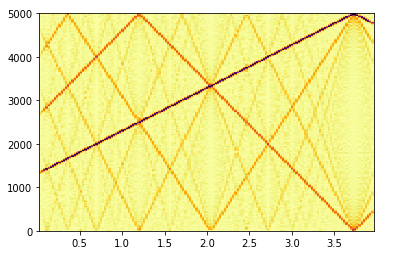
\includegraphics[scale=1]{fig/lab03/lab03_10.png}
		\caption{КПФ сигнала}
	\end{center}
\end{figure}


\subsection{Упражнение 3}

Создадим пилообразный чирп, меняющийся от 2500 до 3000 Гц, на его основе создадим сигнал длительностью 1 секунду и частотой кадров 20 кГц, рапечатаем его спектр

\begin{lstlisting}[language=Python]
signal = SawtoothChirp(start=2500, end=3000)
wave = signal.make_wave(duration=1, framerate=20000)
wave.make_audio()

wave.make_spectrum().plot()
decorate(xlabel='Frequency (Hz)')
\end{lstlisting}

\begin{figure}[H]
	\begin{center}
		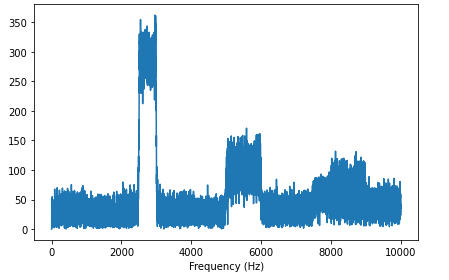
\includegraphics[scale=1]{fig/lab03/lab03_11.png}
		\caption{Спектр сигнала}
	\end{center}
\end{figure}

Из графика видно, что базовая частота колеблется от 2500 до 3000 Hz. Также видны следующие гармоники на частотах от 5000-6000 Hz и от 7500-9000 Hz

\subsection{Упражнение 4}

В музыкальной терминологии «глиссандо» — это нота, которая скользит от одной высоты тона к другой, поэтому она похожа на чириканье. Найдите или сделайте запись глиссандо и постройте его спектрограмму.

Найдем и распечатаем звук глиссандо и распечатаем спектограмму

\begin{lstlisting}[language=Python]
if not os.path.exists('495734__phonosupf__sax-glissando.wav'):
    !wget https://github.com/sergeyfedorov02/Telecom/raw/main/495734__phonosupf__sax-glissando.wav
    
from thinkdsp import read_wave

wave = read_wave('495734__phonosupf__sax-glissando.wav')
wave.make_audio()

wave.make_spectrogram(512).plot(high=5000)
decorate(xlabel='Time (s)', ylabel='Frequency (Hz)')
\end{lstlisting}

\begin{figure}[H]
	\begin{center}
		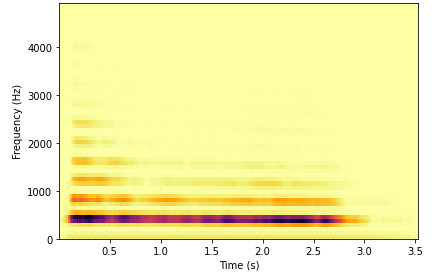
\includegraphics[scale=1]{fig/lab03/lab03_12.png}
		\caption{Спектрограмма сигнала}
	\end{center}
\end{figure}

Видим, что спектограмма очень похожа на наш чирп.

\subsection{Упражнение 5}

Тромбонист может играть глиссандо, выдвигая слайд тромбона и непрерывно дуя. По мере выдвижения ползуна общая длина трубки увеличивается, а результирующий шаг обратно пропорционален длине.
Предполагая, что игрок перемещает слайд с постоянной скоростью, как меняется ли частота со временем?

\noindent Напишите класс TromboneGliss, расширяющий класс Chirp и предоставляет evaluate. Создайте волну, имитирующую тромбон глиссандо от F3 вниз до C3 и обратно до F3. C3 — 262 Гц; F3 есть 349 Гц.

Напишем класс TromboneGliss расширяющий класс Chirp и переопределяющий метод evaluate. Для этого для вычисления частоты используется функция np.linspace, но в аргументы передается не просто начальная и конечная частоты, а единица деленная на эти частоты

\begin{lstlisting}[language=Python]
class TromboneGliss(Chirp):
        
    def evaluate(self, ts):
        l1, l2 = 1.0 / self.start, 1.0 / self.end
        lengths = np.linspace(l1, l2, len(ts))
        freqs = 1 / lengths
        
        dts = np.diff(ts, prepend=0)
        dphis = PI2 * freqs * dts
        phases = np.cumsum(dphis)
        ys = self.amp * np.cos(phases)
        return ys
\end{lstlisting}

Создадим два сигнала-глиссандо от C3 до F3 и обратно, воспроизведем эти звуки, своместим два сигнала в один и построим его спектограмму

\begin{lstlisting}[language=Python]
sig = TromboneGliss(262, 349)
w1 = sig.make_wave(duration=1)
w1.apodize()
w1.make_audio()

sig = TromboneGliss(349, 262)
w2 = sig.make_wave(duration=1)
w2.apodize()
w2.make_audio()

w = w1 | w2
w.make_audio()

sp = wave.make_spectrogram(1024)
sp.plot(high=1000)
decorate(xlabel='Time (s)', ylabel='Frequency (Hz)')
\end{lstlisting}

\begin{figure}[H]
	\begin{center}
		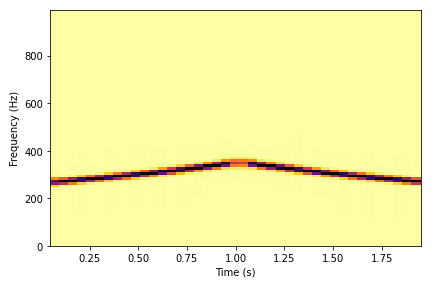
\includegraphics[scale=1]{fig/lab03/lab03_13.png}
		\caption{Спектрограмма сигнала}
	\end{center}
\end{figure}

Как видно из графика и звуков, частота сначала возрастает, а затем спадает до начальной


\subsection{Упражнение 6}

Найдем запись серии гласных звуков и посмотрим на спектограмму

\begin{lstlisting}[language=Python]
if not os.path.exists('code_87778__marcgascon7__vocals.wav'):
    !wget https://github.com/sergeyfedorov02/Telecom/raw/main/code_87778__marcgascon7__vocals.wav
    
wave = read_wave('code_87778__marcgascon7__vocals.wav')
wave.make_audio()

wave.make_spectrogram(1024).plot(high=1000)
decorate(xlabel='Time (s)', ylabel='Frequency (Hz)')
\end{lstlisting}

\begin{figure}[H]
	\begin{center}
		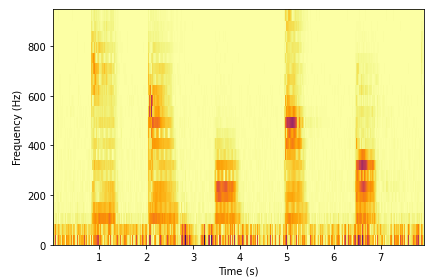
\includegraphics[scale=1]{fig/lab03/lab03_14.png}
		\caption{Спектрограмма гласных звуков}
	\end{center}
\end{figure}

Исходя из графика видно, что фоновый шум - это полоса снизу, а пики - это форманты. Также гласные звуки отличаются по соотношению амплитуд первых двух формант по отношению к основному

\begin{lstlisting}[language=Python]
seg = wave.segment(start=1, duration=0.25)
seg.make_spectrum().plot(high=1000)
decorate(xlabel='Frequency (Hz)')
\end{lstlisting}

\begin{figure}[H]
	\begin{center}
		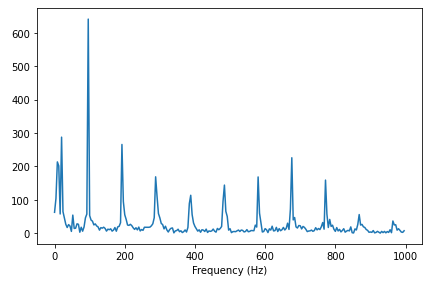
\includegraphics[scale=1]{fig/lab03/lab03_15.png}
		\caption{График частот для звука "ah"}
	\end{center}
\end{figure}

Исходя из графика видно, что основная частота равна 100 Hz, которая соответствует звуку "ah"

\begin{lstlisting}[language=Python]
seg = wave.segment(start=2.2, duration=0.25)
seg.make_spectrum().plot(high=1000)
decorate(xlabel='Frequency (Hz)')
\end{lstlisting}

\begin{figure}[H]
	\begin{center}
		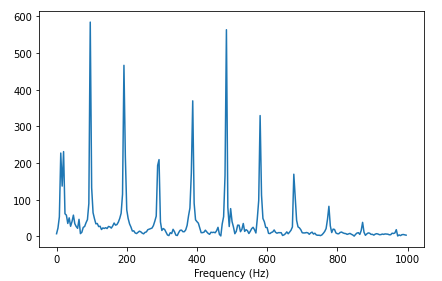
\includegraphics[scale=1]{fig/lab03/lab03_16.png}
		\caption{График частот для звука "eh"}
	\end{center}
\end{figure}

У звука "eh" высокоамплитудная форманта равна 500 Hz

\begin{lstlisting}[language=Python]
seg = wave.segment(start=3.5, duration=0.25)
seg.make_spectrum().plot(high=1000)
decorate(xlabel='Frequency (Hz)')
\end{lstlisting}

\begin{figure}[H]
	\begin{center}
		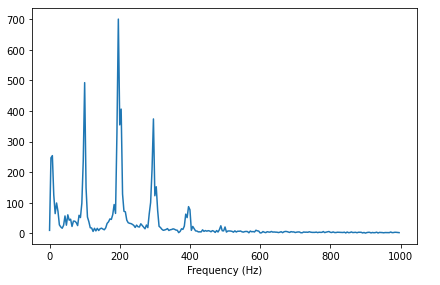
\includegraphics[scale=1]{fig/lab03/lab03_17.png}
		\caption{График частот для звука "ih"}
	\end{center}
\end{figure}

Видно, что у звука "ih" нет высокочастотных составляющих

\begin{lstlisting}[language=Python]
seg = wave.segment(start=5.1, duration=0.25)
seg.make_spectrum().plot(high=1000)
decorate(xlabel='Frequency (Hz)')
\end{lstlisting}

\begin{figure}[H]
	\begin{center}
		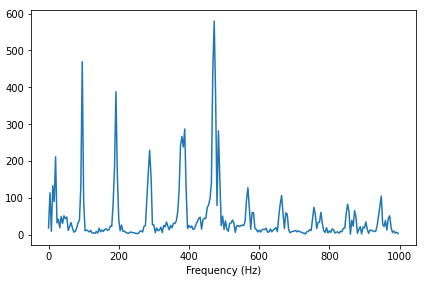
\includegraphics[scale=1]{fig/lab03/lab03_18.png}
		\caption{График частот для звука "oh"}
	\end{center}
\end{figure}

У звука "oh" высокоамплитудная форманта равна 500 Hz

\begin{lstlisting}[language=Python]
seg = wave.segment(start=6.5, duration=0.25)
seg.make_spectrum().plot(high=1000)
decorate(xlabel='Frequency (Hz)')
\end{lstlisting}

\begin{figure}[H]
	\begin{center}
		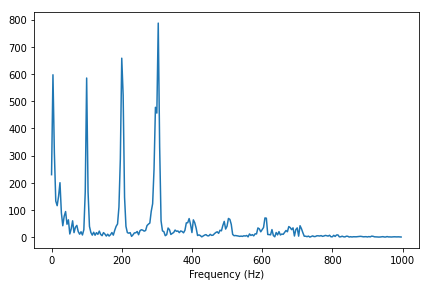
\includegraphics[scale=1]{fig/lab03/lab03_19.png}
		\caption{График частот для звука "oo"}
	\end{center}
\end{figure}

У звука "oo" высокоамплитудная форманта равна 300 Hz


\subsection{Вывод}

В этой работе были расмотрены апериодические сигналы, частотные компоненты которых изменяются во времени. Также в этой главе были рассмотрены спектрограммы - способ визуализации апериодичных сигналов.
